\section{Stack}
E' una struttura dati costruita in SRAM utilizzata dal processore ma anche dal programmatore.
E' una struttura di tipo LIFO (Last-In-First-Out):
\begin{figure}[H]
    \centering
    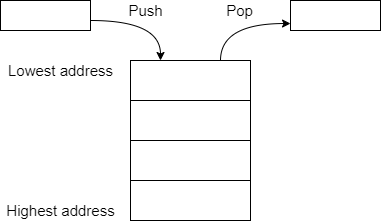
\includegraphics[width=250px]{images/9_Stack/stack.png}
\end{figure}

\subsection{Sub-routine}
E' utilizzata automaticamente dal processore per la chiamata alle sub-routine: supponiamo di avere un pezzo di codice che si occupa di calcolare la radice quadrata alla label RADQ, supponiamo di accedervi tramite l' istruzione JMP:
\begin{verbatim}
    LDI r0, low(900)
    LDI r1, high(900)
        # carico il valore di cui calcolare la sqrt
    JMP radq
        # salto alla procedura
\end{verbatim}
per ritornare al punto in cui ho chiamato la procedura mi servirebbe porre alla fine della procedura un' altra istruzione di salto:
\begin{verbatim}
    JMP foo
\end{verbatim}
Se ora volessi riutilizzare la procedura in un altro punto del codice non potrei perché alla fine di essa mi salterebbe sempre alla fine della prima chiamata!
Per risolvere questo problema sono state introdotte due istruzioni per gestire l' aggancio alle sub-routine:
\begin{itemize}
    \item RCALL radq: salva sullo stack il contenuto del registro PC + 1, sostituisce a PC il valore PC + k + 1.
    E' un salto relativo quindi nell' istruzione ci va un offset, tuttavia a noi basta specificare un' etichetta, l' offset lo calcolerà l'assemblatore per noi.
    Essendo un salto relativo può succedere che non funzioni se l' indirizzo al quale vogliamo andare è troppo lontano.

    \item ICALL radq: salva sullo stack il contenuto del registro PC + 1, sostituisce al registro PC il contenuto del registro Z.
    E' un salto assoluto quindi possiamo specificare l'intero indirizzo al quale vogliamo andare.

    \item CALL radq: salto assoluto che mette l' indirizzo al quale saltare direttamente nell' istruzione.

    \item RET: posto alla fine della procedura riprende il valore salvato sullo stack e lo mette in PC in modo da poter tornare al chiamante.
\end{itemize}
Per eseguire questo genere di operazioni potrebbe bastare salvare il valore in un registro?
No perché non sarebbe possibile innestare varie chiamate l'una dentro l'altra!

\subsection{Utilizzo diretto}
All' avvio del microcontrollore lo stack non è abilitato, va fatto via codice.
Per fare ciò si ricorre a due periferiche: SPL, SPH (SP - Stack Pointer).
All' interno di queste periferiche si inserisce l'indirizzo di inizio dello stack e da quel momento il processore ha lo stack abilitato.

\begin{figure}[H]
    \centering
    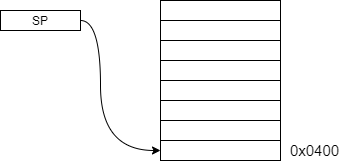
\includegraphics[width=250px]{images/9_Stack/SP.png}
\end{figure}

Possiamo interagire direttamente con lo stack attraverso due istruzioni:
\begin{itemize}
    \item PUSH rs: salva all' indirizzo correntemente puntato da SP il valore del registro passato e decrementa il valore di SP di 1 (la pila cresce verso indizzi più bassi)
    \item POP rd: decrementa il valore di SP e posiziona nel registro passato il valore puntato da SP
    (la pila decresce verso indirizzi più alti)
\end{itemize}

Di solito allo stack si riserva la parte finale della SRAM, un esempio di inizializzazione sarebbe dunque:
\begin{verbatim}
    LDI r16, low(0x085F)
    LDI r17, high(0x085F)
    OUT 0x3D, r16
    OUT 0x3E, r17
\end{verbatim}

Usare gli indirizzi raw è abbastanza caotico, la ATMEL e quindi l'ambiente di sviluppo, mettono a disposizione delle etichette già esistenti per tutti quei valori utili all' interno della programmazione, possiamo pertanto utilizzarli:
\begin{verbatim}
    LDI r16, low(RAMEND)
    LDI r17, high(RAMEND)
    OUT SPL, r16
    OUT SPH, r17
\end{verbatim}

\subsubsection{Swap di due registri}
Un esempio di utilizzo è quello dello swap di due registri:
\begin{verbatim}
    PUSH r10
    MOV r0, r1
    POP r1
    
    
    PUSH r0
    PUSH r1
    POP r0
    POP r1
\end{verbatim}

\subsection{Leggere il valore di PC}
Se per qualche motivo dovesse essere importante leggere il valore di PC si può usare:
\begin{verbatim}
    RCALL 0
        # salva sullo stack PC + 1
        # cioè l'indirizzo della prossima istruzione
    POP r0
    POP r1
\end{verbatim}




